\documentclass[a4paper]{article}
\usepackage[T1]{fontenc} 
\usepackage[utf8]{inputenc}
\usepackage[pdftex,scale={.8,.8}]{geometry}
\usepackage{graphicx}
\usepackage[czech]{babel}
\usepackage{enumitem}
\usepackage{titlesec}
\usepackage{minted}
\usepackage[unicode]{hyperref}
\hypersetup{
    colorlinks,
    linkcolor=black,
}

\begin{document}

    \begin{titlepage}
        \begin{center}
            
            
\includegraphics[scale=0.1,keepaspectratio]{fig/logo_cz.png}
            
            \vspace{3cm}
           
            {\textbf{\Huge ISS - Systémy a signály}}
            
            \vspace{1cm}
            
            {\textbf{\LARGE Protokol k projektu}}
            
            \vspace{0.25cm}
            
            {\LARGE 2020/2021}
            
            \vspace{2cm}
            
            \Large
            \begin{tabular}{l l}
    				Karel Norek & xnorek01
    		\end{tabular}
            
            \vfill
        \end{center}
    
    \end{titlepage}
    \large
    \pagenumbering{arabic}
    \setcounter{page}{1}
    \textbf{Úvod}
    \newline
    Pro spuštění na Merlinovi je nutné doinstalovat potřebné knihovny pomocí příkazu \textbf{pip install -r requirements.txt}
    \begin{enumerate}
        \item \textbf{Tón s rouškou a bez}
        
        \vspace{0.5cm}
        
        Pro nahrání nahrávek jsem použil aplikaci Voice Recorder na Androidu.
            \begin{table}[!ht]
                \renewcommand{\arraystretch}{1.5}
                \centering
                \begin{tabular}{|l|l|}
                \hline
                    Input File & maskoff\_tone.wav \\ \hline
                    Channels & 1\\ \hline
                    Sample Rate & 16000\\ \hline
                    Precision & 16-bit\\ \hline
                    Duration & 00:00:03.84 = 61418 samples ~ 287.897 CDDA sectors\\ \hline
                    File Size & 123k\\ \hline
                    Bit Rate & 256k\\ \hline
                    Sample Encoding & 16-bit Signed Integer PCM\\
                \hline
                \end{tabular}
                \caption{Tón bez roušky}
                \label{tab:mask_off_tone}
            \end{table}
         
            \begin{table}[!ht]
                \renewcommand{\arraystretch}{1.5}
                \centering
                \begin{tabular}{|l|l|}
                \hline
                    Input File & maskon\_tone.wav \\ \hline
                    Channels & 1\\ \hline
                    Sample Rate & 16000\\ \hline
                    Precision & 16-bit\\ \hline
                    Duration & 00:00:03.68 = 58858 samples ~ 275.897 CDDA sectors\\ \hline
                    File Size & 118k\\ \hline
                    Bit Rate & 256k\\ \hline
                    Sample Encoding & 16-bit Signed Integer PCM\\
                \hline
                \end{tabular}
                \caption{Tón s rouškou}
                \label{tab:maask_on_tone}
            \end{table}
        \item \textbf{Věty s rouškou a bez}
            \begin{table}[!ht]
                \renewcommand{\arraystretch}{1.5}
                \centering
                \begin{tabular}{|l|l|}
                \hline
                    Input File & maskoff\_sentence.wav \\ \hline
                    Channels & 1\\ \hline
                    Sample Rate & 16000\\ \hline
                    Precision & 16-bit\\ \hline
                    Duration & 00:00:02.96 = 47338 samples ~ 221.897 CDDA sectors\\ \hline
                    File Size & 94.7k\\ \hline
                    Bit Rate & 256k\\ \hline
                    Sample Encoding & 16-bit Signed Integer PCM\\
                \hline
                \end{tabular}
                \caption{Věta bez roušky}
                \label{tab:mask_off_sentence}
            \end{table}
        \newpage
            \begin{table}[!ht]
                \renewcommand{\arraystretch}{1.5}
                \centering
                \begin{tabular}{|l|l|}
                \hline
                    Input File & maskon\_sentence.wav \\ \hline
                    Channels & 1\\ \hline
                    Sample Rate & 16000\\ \hline
                    Precision & 16-bit\\ \hline
                    Duration & 00:00:03.04 = 48618 samples ~ 227.897 CDDA sectors\\ \hline
                    File Size & 97.3k\\ \hline
                    Bit Rate & 256k\\ \hline
                    Sample Encoding & 16-bit Signed Integer PCM\\
                \hline
                \end{tabular}
                \caption{Věta s rouškou}
                \label{tab:mask_onf_sentence}
            \end{table}
        \item \textbf{Zpracování nahrávek a vytvoření rámců} 
        
        \vspace{0.25cm}
        
        Pro načtení nahrávky jsem použil knihovnu scipy.wavfile.. \newline
        Musel jsem nahrávku normalizovat pomocí \textbf{data = data / 2**15} \newline
        Pro ustřednění jsem použil vzorec: $x[n]$ - $\overline{x}$
        
        \vspace{0.25cm}
        
        Výpočet velikosti rámce jsem provedl následovně:
        \begin{minted}[gobble=12]{python}
          
            frames = [data[i*sr*10 : i*10*sr + 20*sr] for i in range(100)]
        \end{minted}
        sr je počet vzorků v jedné ms. i*sr*10 vypočítá, kde začíná prvních 10 ms rámce. Po přičtení 20*sr dostaneme konec rámce dlouhého 20 ms. Díky iteraci se rámce budou zároveň překrývat. Touto metodou nám vznikne 100 rámců.
        
        \vspace{0.25cm}
        \textbf{Rámec 70 z obou tónů:}
     
            \begin{figure}[!ht]
    	        \centering
    	        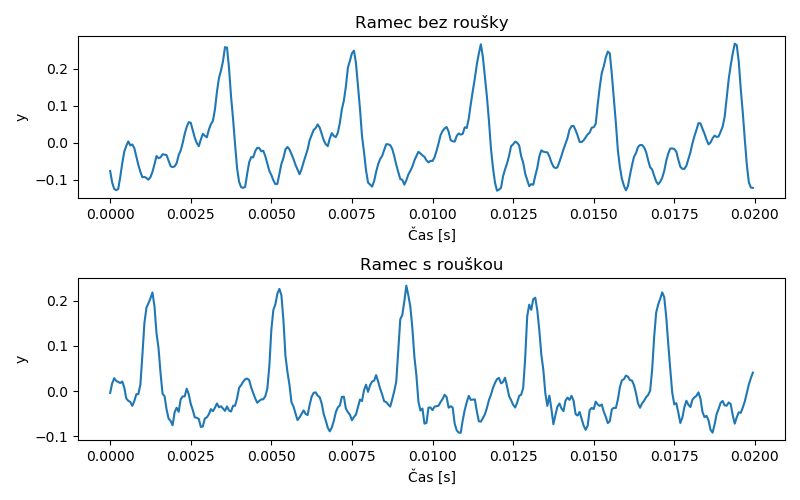
\includegraphics[scale=0.8,keepaspectratio]{fig/frames.png}
    	        \label{fig:frames}
	        \end{figure}
        \newpage    
        
        \item \textbf{Klipování, Autokorelace a porovnání rámců}
        
        \vspace{0.25cm}
        
        Pro ukázku klipování a autokorelace jsem vybral rámec 70 (index 69) stejný jako u úkolu 3. Klipování a autokorelaci jsem provedl podle zadání. Základní frekvenci jsem poté vypočítal jako $F_0 = 1/T$. Kde $T = lag/fs$.
            \begin{figure}[!ht]
    	        \centering
    	        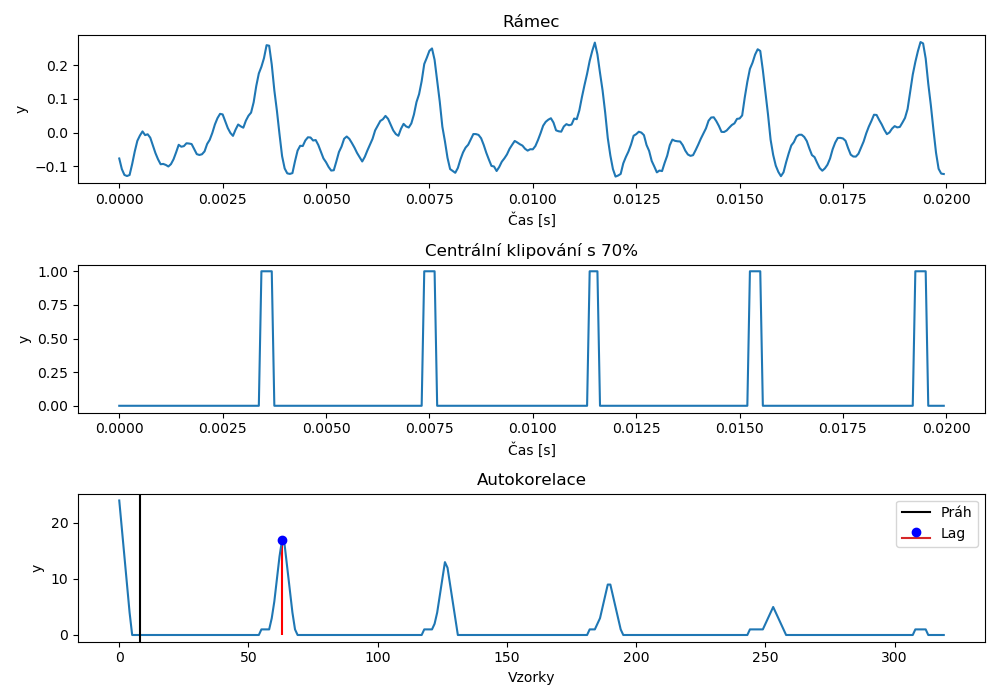
\includegraphics[scale=0.65,keepaspectratio]{fig/clip_correlate.png}
    	        \label{fig:clips}
	        \end{figure}
	        
	        \begin{figure}[!ht]
    	        \centering
    	        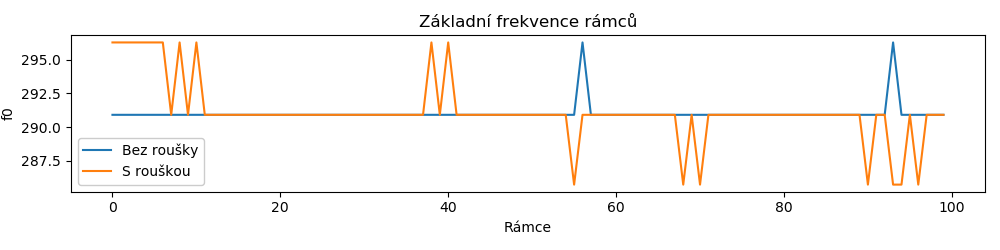
\includegraphics[scale=0.65,keepaspectratio]{fig/ramce.png}
    	        \label{fig:ramce}
	        \end{figure}
	        
	   \textbf{Střední hodnota pro rámce s rouškou:} 291.1380471380471 Hz \newline
	   \textbf{Střední hodnota pro rámce bez roušky:} 291.01683501683516 Hz \newline
	   \textbf{Rozptyl pro rámce s rouškou:} 5.029017123293211 Hz \newline
	   \textbf{Rozptyl pro rámce bez roušky:} 0.5688308449251173 Hz \newline
	   
	   Otazka: Snížit změnu f0 při lagu bychom mohli tak, že se frekvencí přiblížíme vzorkovací frekvenci a tím pádem nebudeme mít tak rozdílné výsledky f0.
	   
	    
	    \item \textbf{Spektrogramy}
	    
	    \vspace{0.25cm}
	    
	    Pro tento úkol jsme měli implementovat vlastní DFT.
	    
	    \begin{figure}[!ht]
    	        \centering
    	        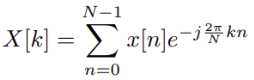
\includegraphics[scale=0.65,keepaspectratio]{fig/DFT.png}
    	        \label{fig:DFT}
	   \end{figure}
	   \textbf{Implementace:}
	    \begin{minted}[gobble=12]{python}
            def myDFT(frame):
                z = np.zeros(1024)
                z[:320] = np.copy(frame)
                array =[]
                for k in range(1024):
                    value = 0
                    for t in range(1024):
                        value += z[t] * (np.e ** (-2 * np.pi * 1j * t * k/1024))
                    array.append(value)
                return array
            
            myDFT_off = []
            myDFT_on = []
            for i in range(len(frames_off)):
                myDFT_off.append(myDFT(frames_off[i]))
                myDFT_on.append(myDFT(frames_on[i]))
        \end{minted}
	    Nicméně svoji implementaci nepoužívám, protože je pomalejší než existující \textbf{numpy.fft.fft}. V kódu ji mám vloženou do podmínky \textbf{if 0:} aby mi nezpomalovala zbytek kódu.
	    
	        \begin{figure}[!ht]
    	        \centering
    	        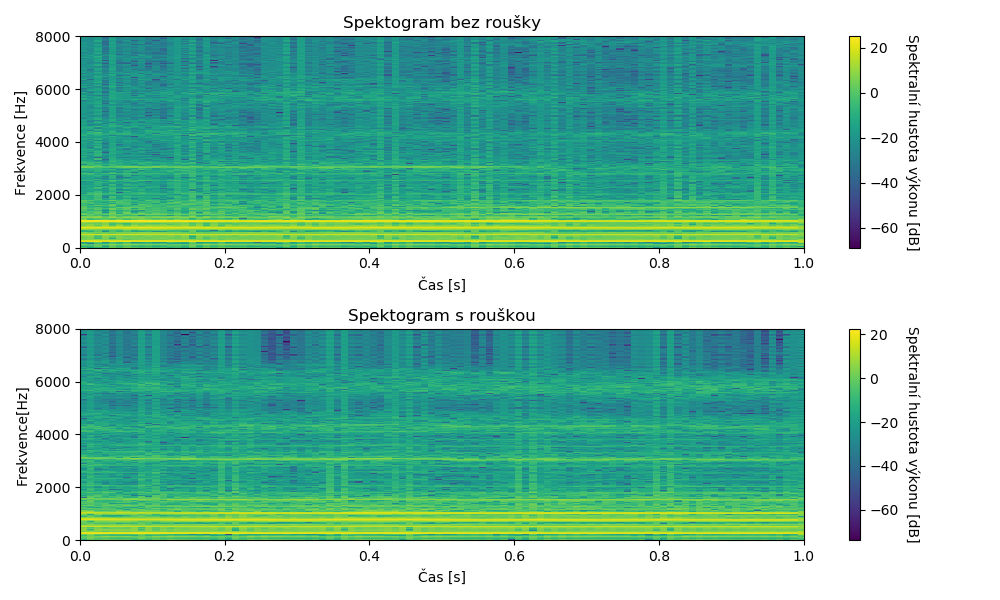
\includegraphics[scale=0.65,keepaspectratio]{fig/Spektogram.png}
    	        \label{fig:spec}
	        \end{figure}
	   \newpage
	    \item \textbf{Frekvenční charakteristika roušky}
	    
	    \vspace{0.25cm}
	    \textbf{Vztah pro výpočet  $H(e^j^\omega)$:}
	    
	    \[ H(e^j^\omega) = \frac{B(e^j^\omega)}{A(e^j^\omega)} = \frac{b(0)e^-^j^\omega^\cdot^0 + b(1)e^-^j^\omega^\cdot^1 + ... + b(n)e^-^j^\omega^\cdot^n}{a(0)e^-^j^\omega^\cdot^0 + a(1)e^-^j^\omega^\cdot^1 + ... + a(m)e^-^j^\omega^\cdot^m} \]
	    
	    B jsou rámce s rouškou po DFT. A jsou rámce bez roušky po DFT.
	    
	    Filtr je symetrický. Proto budeme brát v potaz pouze 512 prvků. Tím že jsme vydělili hodnoty B a A jsme dostali pouze charakteristiku roušky - jediný rozdíl v nahravkách. Dolní propusť
	    
	    \vspace{0.25cm}
	        \begin{figure}[!ht]
    	        \centering
    	        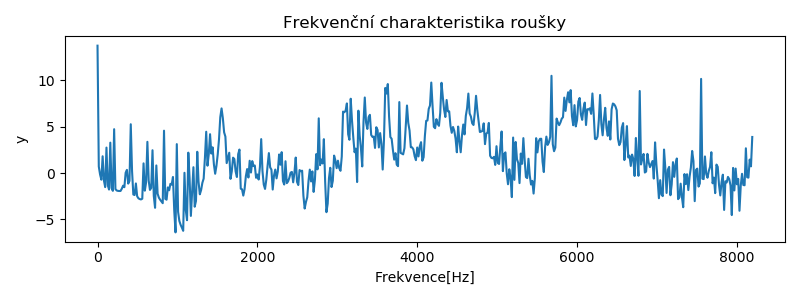
\includegraphics[scale=0.7,keepaspectratio]{fig/freq_char.png}
    	        \label{fig:freq}
	        \end{figure}
	    \item \textbf{Impulzivní odezva}
	    
	    \vspace{0.25cm}
	     Pro tento úkol jsme měli implementovat vlastní IDFT.
	     \begin{figure}[!ht]
    	        \centering
    	        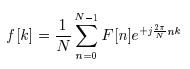
\includegraphics[scale=0.65,keepaspectratio]{fig/IDFT.png}
    	        \label{fig:IDFT}
	   \end{figure}
	   \newline
	   \textbf{Implementace:}
	    \begin{minted}[gobble=12]{python}
            def myIDFT(frame):
                z = np.zeros(1024)
                z[:512] = np.copy(frame)
                array =[]
                for k in range(1024):
                    value = 0
                    for t in range(1024):
                        value += z[t] * (np.e ** (2 * np.pi * 1j * t * k/1024))
                    value = value / 1024
                    array.append(value)
                return array
            
            myIDFT_off = myIDFT(H[:512])
            myIDFT_on = myIDFT(H[:512])
        \end{minted}
       
	    Nicméně svoji implementaci zase nepoužívám, protože je pomalejší než existující \textbf{numpy.fft.ifft}. V kódu ji mám vloženou do podmínky \textbf{if 0:} aby mi nezpomalovala zbytek kódu. \newline
	     Do IDFT dávám pouze 512 vzorků z úkolu 6, protože s 1024 vzorky mi nakonec rouška zesilovala. Proto jsem vzal půlku protože 2. půlka je symetrická.
	        \begin{figure}[!ht]
    	        \centering
    	        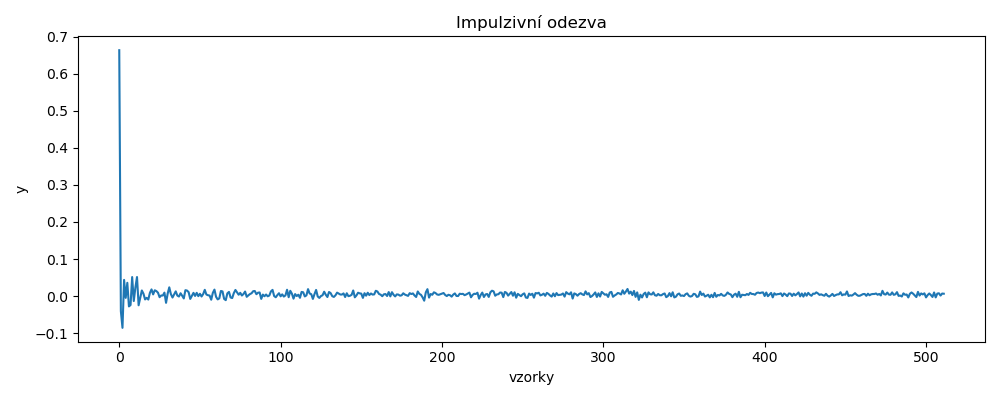
\includegraphics[scale=0.7,keepaspectratio]{fig/odezva.png}
    	        \label{fig:odezva}
	        \end{figure}
	    \item \textbf{Simulace roušky}
	    
	    \vspace{0.25cm}
	    
	    Využijeme filtr k simulaci roušky u nahrávky bez roušky. Pro simulaci je používaná funkce lfilter.
	        \begin{figure}[!ht]
    	        \centering
    	        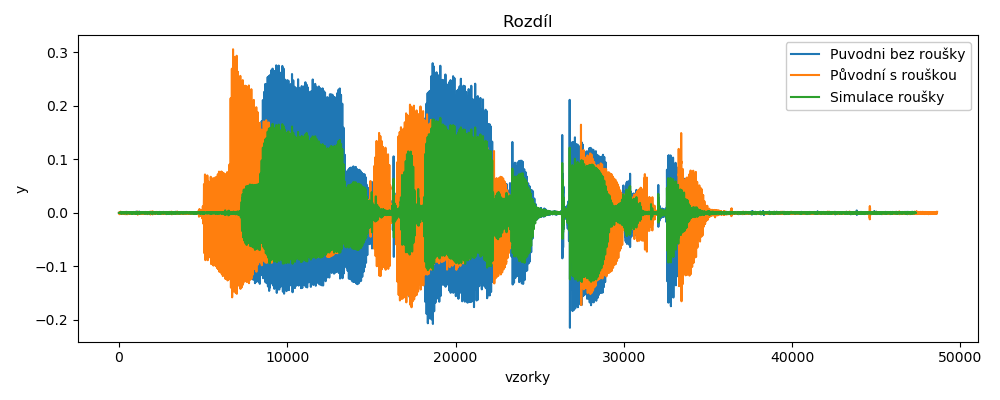
\includegraphics[scale=0.7,keepaspectratio]{fig/rozdil.png}
    	        \label{fig:rozdily}
	        \end{figure}
	        
	   Signál simulované roušky je velice podobný tomu pravému, ale nahravky nejsou stejně dlouhé. Původní věta s rouškou se řekla pomaleji proto uplně nesedí na sobě, ale s trochou představivosti můžeme vidět že jsou jinak rozsahově velmi pdobné. Nejvíce se podobají když je signál tišší a nejméně kde je zase naopak signal moc hlasitý.
	
	   \item \textbf{Závěr}
	   
	   \vspace{0.25cm}
	   
	   Podle mě moje řešení funguje. Nahrávku jsem měl v pořádku, ale to mi ztížilo hledání n-násobného lagu. Co bych si určitě vytkl, je nepřesnost vět s rouškou a bez. Jedna je rychlejší a druhá pomalejší, takže se špatně porovnává simulovaná věta.
	   \setcounter{enumi}{10}
	   \item \textbf{Okénková funkce}
	   \newline
	   Jako okénekovou funkci jsem si vybral funkci Hamming. Grafy jsem čerpal z oficiální dokumentace pro funkci numpy.hamming. 
	   \begin{figure}[!ht]
    	        \centering
    	        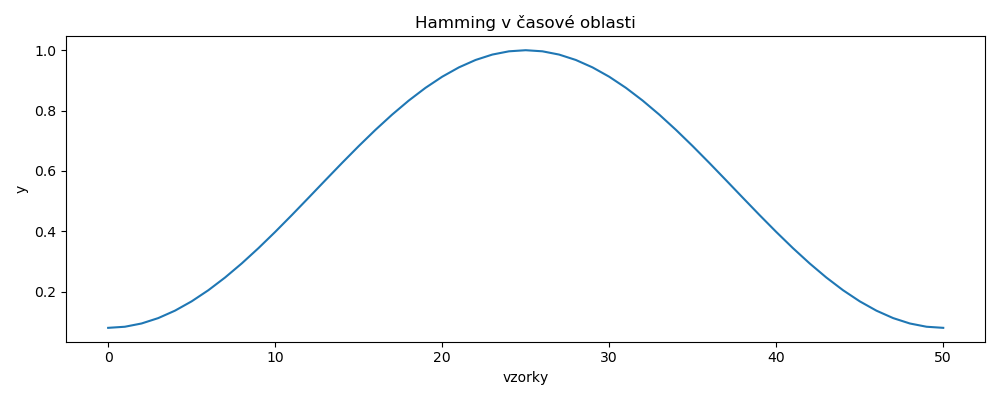
\includegraphics[scale=0.65,keepaspectratio]{fig/hamming.png}
    	        \label{fig:hamm}
	        \end{figure}
	        \begin{figure}[!ht]
    	        \centering
    	        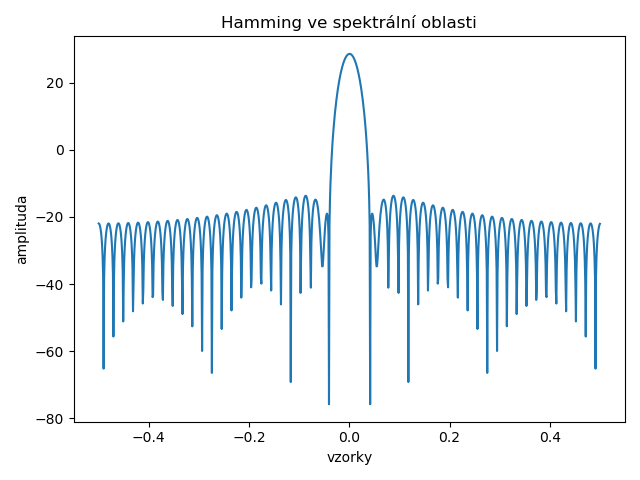
\includegraphics[scale=0.65,keepaspectratio]{fig/hamming_DFT.png}
    	        \label{fig:hamm}
	        \end{figure}
	        \begin{figure}[!ht]
    	        \centering
    	        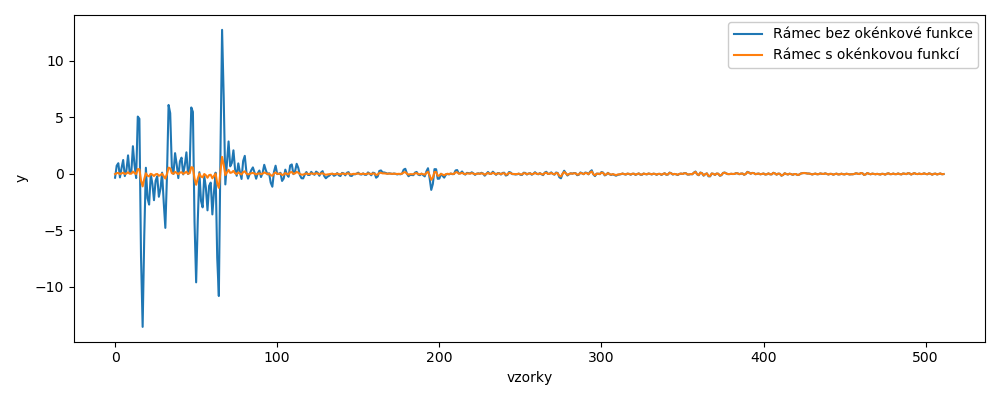
\includegraphics[scale=0.7,keepaspectratio]{fig/hamming_porovnani.png}
    	        \label{fig:hamm}
	        \end{figure}
	        
	   Okénková funkce je užitečná, protože nám umožní distribuovat "Spectral leakage" podle potřeby.
	   \newpage
	   \setcounter{enumi}{12}
	   \item \textbf{Stejná základní frekvence}
	   
	   \vspace{0.25cm}
	   
	    \begin{figure}[!ht]
    	        \centering
    	        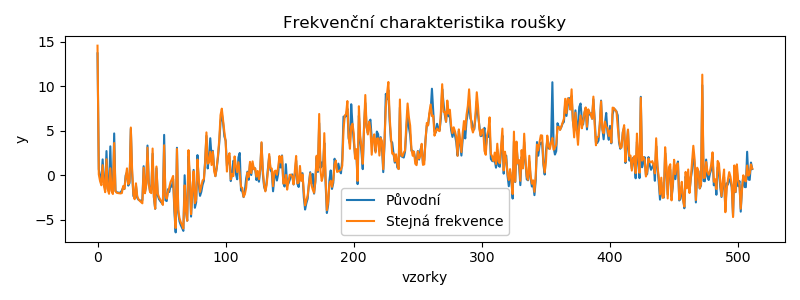
\includegraphics[scale=0.7,keepaspectratio]{fig/freq_char_same.png}
    	        \label{fig:freq_same}
	        \end{figure}
	        Můžeme vidět, že charakteristika pouze z rámcu se stejnou frekvencí nabývají menších hodnot. To je způsobeno tím, že používáme více podobné rámce, ale také méně hodnot.
    \end{enumerate}
    

\end{document}
